\documentclass[12pt,a4paper]{article}
\usepackage[utf8]{inputenc}
\usepackage[T1]{fontenc}
\usepackage[spanish,es-nodecimaldot]{babel}
\usepackage{geometry}
\usepackage{xcolor}
\usepackage{graphicx}
\usepackage{booktabs}
\usepackage{longtable}
\usepackage{listings}
\usepackage{fancyvrb}
\usepackage{float}
\usepackage{hyperref}
\usepackage{tikz}
\usetikzlibrary{arrows.meta,positioning,fit,shapes.geometric}

\geometry{margin=2.4cm}
\hypersetup{colorlinks=true,linkcolor=blue!50!black,urlcolor=blue!60!black}
\definecolor{unsa}{HTML}{1A3A5C}
\definecolor{accent}{HTML}{C0392B}
\definecolor{soft}{HTML}{F0F4F8}
\definecolor{codegreen}{HTML}{166534}

\lstdefinestyle{code}{
  basicstyle=\ttfamily\small,
  backgroundcolor=\color{soft},
  frame=single,
  breaklines=true,
  showstringspaces=false,
  keywordstyle=\color{unsa}\bfseries,
  commentstyle=\color{codegreen},
  stringstyle=\color{accent}
}
\lstset{style=code}

\newcommand{\evidence}[2]{%
  \subsubsection*{#1}
  \IfFileExists{evidence/#2}{\VerbatimInput[fontsize=\scriptsize]{evidence/#2}}%
  {\fbox{\parbox{0.94\linewidth}{Evidencia pendiente. Ejecutar
  \texttt{powershell -File scripts/capture-evidence.ps1}.}}}
}

\title{\textbf{Sistema de matrícula universitario escalable y tolerante a fallos sobre Kubernetes}\\[0.4cm]
\large Proyecto Final de Unidad --- Cloud Computing}
\author{Universidad Nacional de San Agustín de Arequipa\\
\textit{Integrantes: completar nombres y CUI}}
\date{2026}

\begin{document}
\maketitle
\thispagestyle{empty}
\begin{center}
\vfill
\textbf{Escenario académico inspirado en la UNSA}\\[0.3cm]
Frontend Vue 3 --- API Node/Express --- PostgreSQL --- Redis --- Kubernetes
\vfill
\end{center}
\newpage

\tableofcontents
\newpage

\section{Resumen ejecutivo}
Se implementó una arquitectura cloud-native para un sistema de matrícula universitaria.
La aplicación constituye el caso de negocio, mientras Kubernetes es el componente central
de la evaluación. La solución demuestra balanceo entre réplicas, escalamiento horizontal
por CPU, recuperación automática, persistencia, configuración desacoplada, caché,
actualizaciones progresivas y backups programados.

La evaluación se realiza mediante experimentos reproducibles. Cada experimento define un
estado inicial, una acción, una observación y evidencia obtenida directamente del clúster.
Además, se desarrolló un dashboard de consola para facilitar la exposición y explicar qué
ocurre ante una falla y cómo diagnosticarla.

\section{Objetivos}
\subsection{Objetivo general}
Implementar y evaluar una arquitectura cloud-native para un sistema de matrícula
universitario utilizando Kubernetes, demostrando escalabilidad horizontal, tolerancia a
fallos, persistencia, configuración externa y despliegues sin interrupción mediante
experimentos controlados.

\subsection{Objetivos específicos}
\begin{itemize}
  \item Contenerizar frontend y backend y desplegarlos con réplicas administradas.
  \item persistir los datos de PostgreSQL independientemente del ciclo de vida del Pod;
  \item reducir consultas repetidas mediante Redis;
  \item escalar el backend de dos a cinco réplicas utilizando métricas de CPU;
  \item comprobar self-healing, probes, rolling update y rollback;
  \item automatizar backups persistentes y recopilar evidencia técnica.
\end{itemize}

\section{Arquitectura}
\begin{figure}[H]
\centering
\begin{tikzpicture}[
  node distance=8mm and 12mm,
  box/.style={draw=unsa,rounded corners,fill=blue!5,minimum width=35mm,minimum height=9mm,align=center},
  data/.style={draw=accent,rounded corners,fill=red!5,minimum width=35mm,minimum height=9mm,align=center},
  arr/.style={-{Latex[length=2.5mm]},thick,color=unsa}
]
\node[box] (users) {Estudiantes};
\node[box,below=of users] (ingress) {Ingress / Gateway};
\node[box,below=of ingress] (frontsvc) {frontend-service};
\node[box,below=of frontsvc] (front) {Frontend Pod\\Vue + Nginx};
\node[box,below=of front] (backsvc) {backend-service};
\node[box,below left=of backsvc] (b1) {Backend B1};
\node[box,below right=of backsvc] (bn) {Backend B2...B5};
\node[data,below=18mm of b1] (pg) {PostgreSQL\\StatefulSet + PVC};
\node[data,below=18mm of bn] (redis) {Redis\\Deployment};
\node[data,below=of pg] (backup) {CronJob\\PVC backups};
\draw[arr] (users)--(ingress);
\draw[arr] (ingress)--(frontsvc);
\draw[arr] (frontsvc)--(front);
\draw[arr] (front)--node[right]{\scriptsize /api}(backsvc);
\draw[arr] (backsvc)--(b1);
\draw[arr] (backsvc)--(bn);
\draw[arr] (b1)--(pg);
\draw[arr] (b1)--(redis);
\draw[arr] (bn)--(pg);
\draw[arr] (bn)--(redis);
\draw[arr] (pg)--(backup);
\end{tikzpicture}
\caption{Arquitectura lógica de la solución.}
\end{figure}

\subsection{Flujo de una solicitud}
El usuario accede al punto de entrada HTTP. El tráfico llega al frontend, cuyo Nginx sirve
la aplicación Vue y reenvía las rutas \texttt{/api} al Service del backend. El Service
distribuye conexiones entre Pods disponibles. El backend consulta PostgreSQL para datos
transaccionales y Redis para resultados cacheables.

\section{Componentes desarrollados}
\begin{longtable}{p{0.22\linewidth}p{0.23\linewidth}p{0.46\linewidth}}
\toprule
Componente & Tecnología & Responsabilidad \\
\midrule
Frontend & Vue 3 + Nginx & Cursos, vacantes, matrícula, cursos inscritos y visualización de distribución. \\
Backend & Node.js + Express & API REST, transacciones, caché, health checks e identificación del Pod. \\
Base de datos & PostgreSQL 15 & Estudiantes, cursos, vacantes y matrículas. \\
Caché & Redis 7 & Caché de cursos con invalidación posterior a una matrícula. \\
Plataforma & Kubernetes & Scheduling, Service discovery, self-healing, HPA, persistencia y Jobs. \\
Pruebas & k6 & Carga por etapas, latencia, errores y carga CPU controlada. \\
Operación & PowerShell & Dashboard, diagnóstico y ejecución guiada de demostraciones. \\
\bottomrule
\end{longtable}

\section{Recursos Kubernetes}
\begin{longtable}{p{0.27\linewidth}p{0.64\linewidth}}
\toprule
Recurso & Uso en el proyecto \\
\midrule
Namespace & Aislamiento lógico en \texttt{unsa-matricula}. \\
Deployments & Frontend, backend y Redis; backend inicia con dos réplicas. \\
StatefulSet & PostgreSQL conserva identidad estable como \texttt{postgres-0}. \\
Services & Descubrimiento estable sin depender de direcciones IP de Pods. \\
Ingress & Entrada HTTP por nombre de host. \\
ConfigMap & Hosts, puertos, base de datos y URL interna del backend. \\
Secret & Credenciales de PostgreSQL inyectadas como variables. \\
PVC & Volúmenes separados para datos y backups. \\
HPA & Escalamiento del backend entre 2 y 5 Pods con objetivo de CPU de 50\%. \\
Probes & Startup, readiness y liveness para controlar el ciclo de vida. \\
CronJob & Ejecución de \texttt{pg\_dump} cada cinco minutos con retención de diez archivos. \\
\bottomrule
\end{longtable}

\section{Decisiones técnicas relevantes}
\subsection{Matrícula concurrente}
La matrícula se ejecuta dentro de una transacción. La fila del curso se bloquea con
\texttt{SELECT ... FOR UPDATE}; de esta forma dos solicitudes concurrentes no pueden
consumir la última vacante simultáneamente. La restricción única evita duplicar una
matrícula por estudiante y curso.

\subsection{Caché e invalidación}
\texttt{GET /courses} consulta primero Redis. Ante un miss se consulta PostgreSQL y se
almacena el resultado durante 30 segundos. Después de una matrícula se eliminan las claves
afectadas para no presentar vacantes obsoletas.

\subsection{Escalamiento reproducible}
Se incorporó \texttt{GET /load}, limitado a 100 ms, que realiza trabajo criptográfico
controlado. Esto permite incrementar CPU de manera segura y reproducible durante k6, sin
confundir el experimento con saturación de la base de datos.

\subsection{Backup persistente}
El CronJob monta \texttt{postgres-backups-pvc}; por tanto, el dump permanece después de
que termina el Pod del Job. Se conservan los diez backups más recientes.

\section{Dashboard de consola}
El archivo \texttt{scripts/dashboard.ps1} centraliza la exposición. Presenta la
arquitectura, salud de Pods, réplicas del HPA, CPU, memoria, reinicios y eventos recientes.
También analiza estados no saludables y propone \texttt{describe} y revisión de logs.

\begin{lstlisting}[language=bash,caption={Inicio del centro de demostración}]
powershell -ExecutionPolicy Bypass -File scripts/dashboard.ps1
\end{lstlisting}

Sus opciones ejecutan balanceo, caché, self-healing, persistencia y backup sin tener que
memorizar todos los comandos durante la exposición.

\begin{figure}[H]
\centering
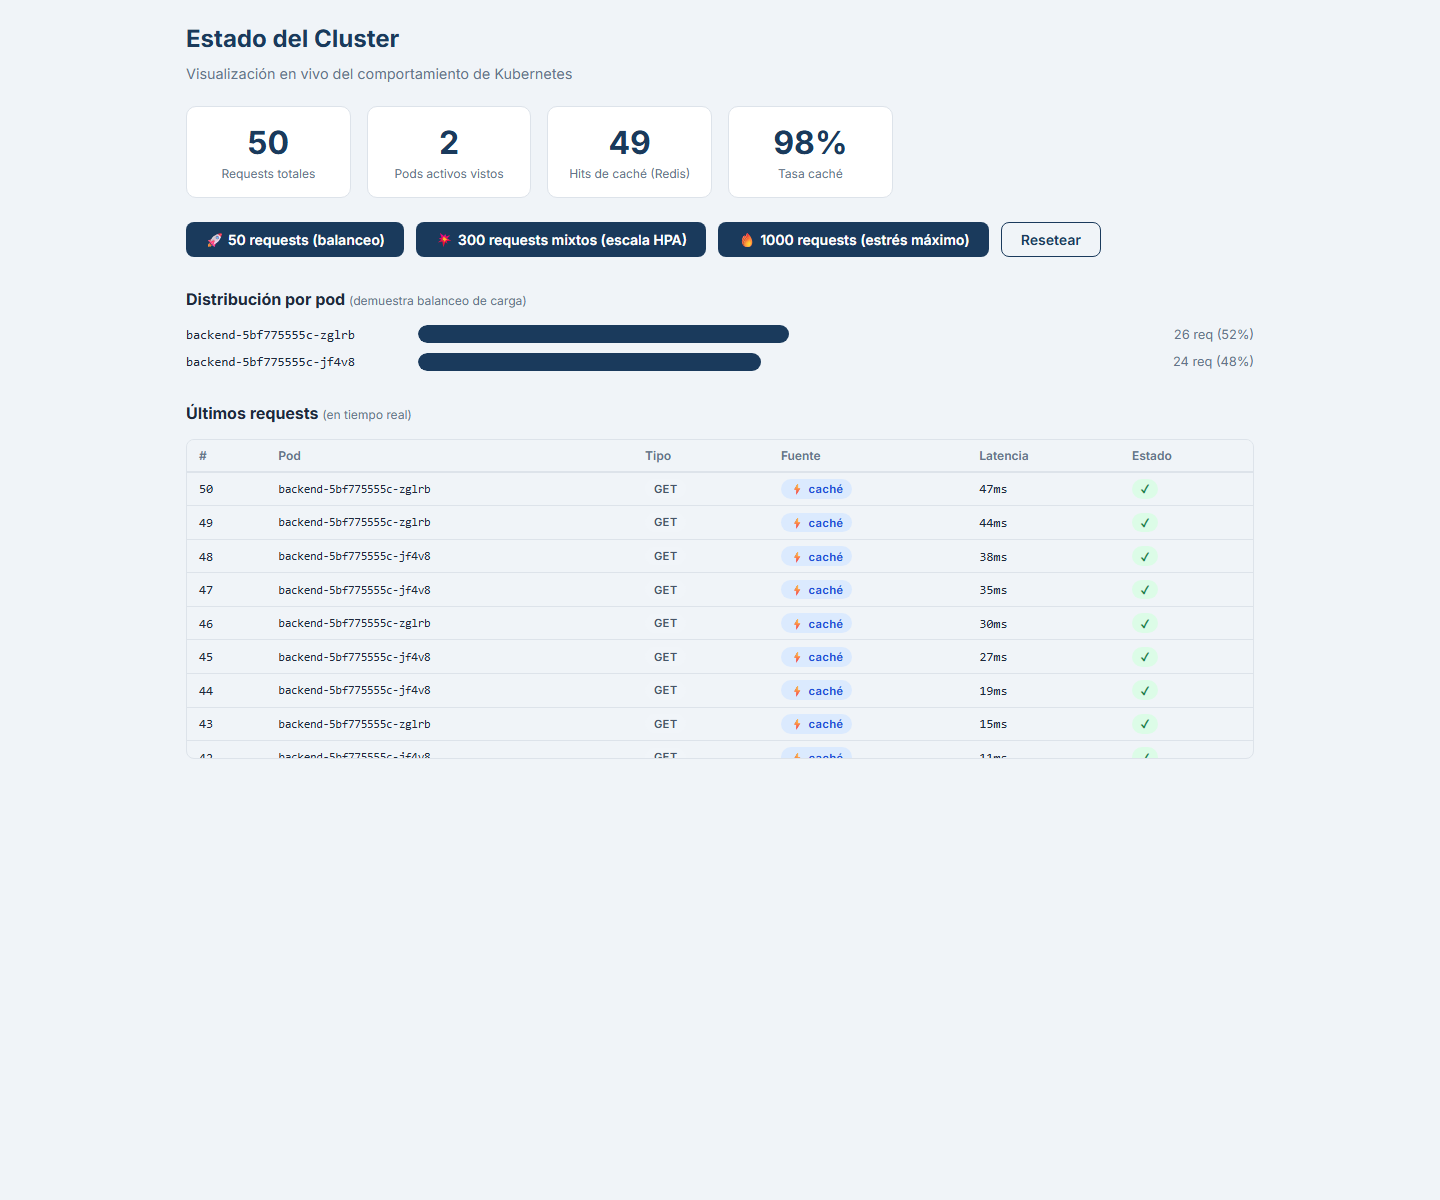
\includegraphics[width=0.92\linewidth]{evidence/02-cluster-dashboard.png}
\caption{Dashboard web mostrando 50 solicitudes distribuidas entre dos Pods.}
\end{figure}

\begin{figure}[H]
\centering
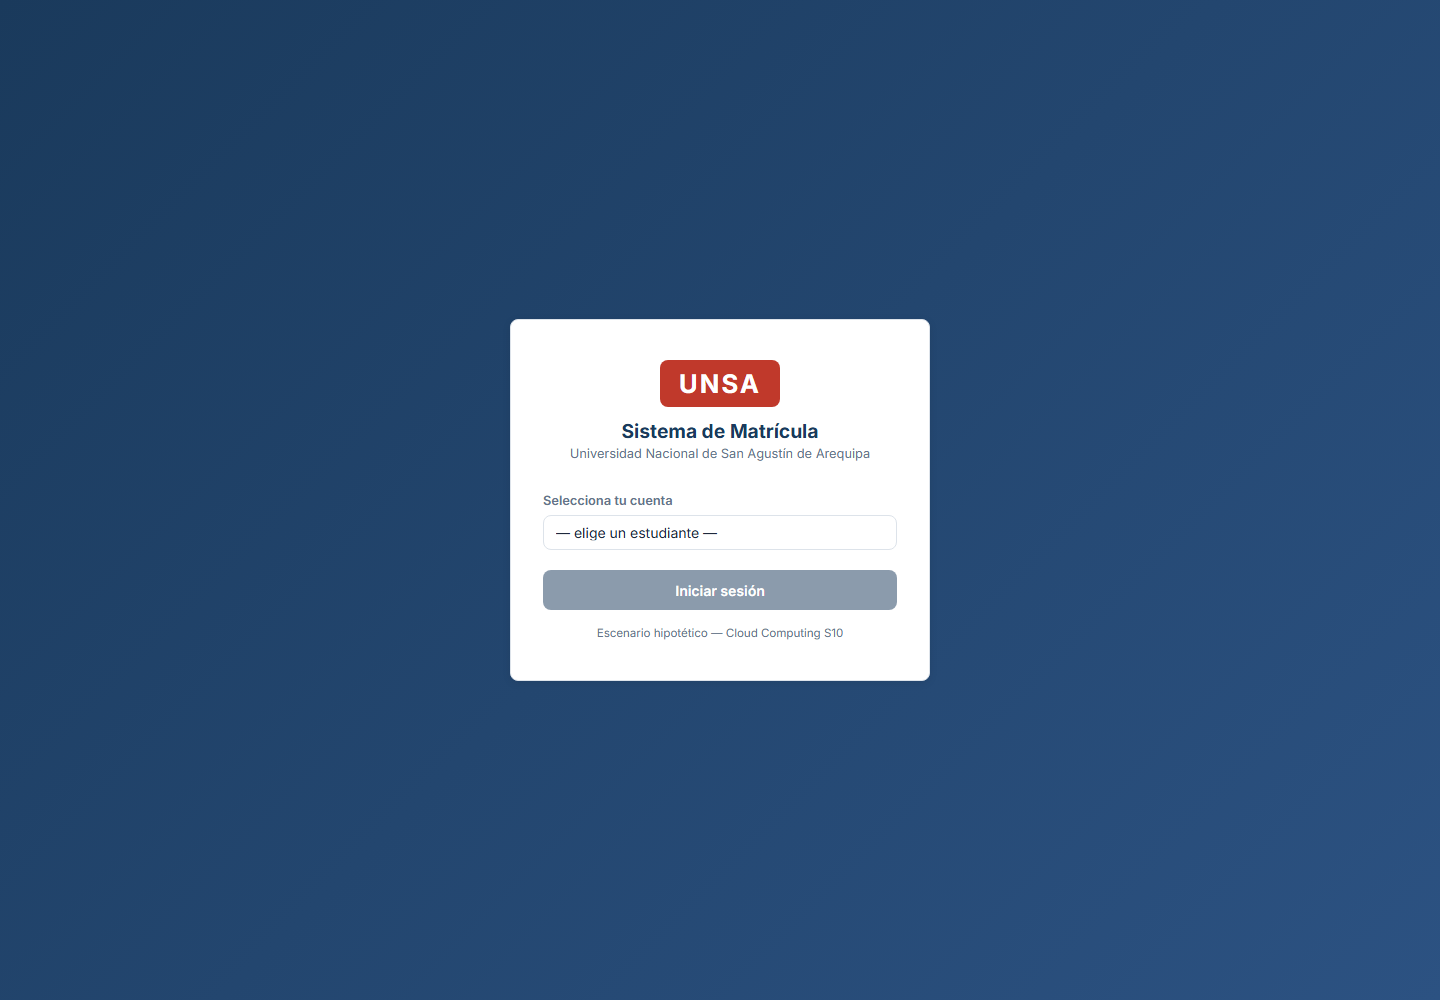
\includegraphics[width=0.82\linewidth]{evidence/01-login.png}
\caption{Punto de entrada del sistema de matrícula desplegado.}
\end{figure}

\section{Metodología experimental}
\begin{longtable}{p{0.16\linewidth}p{0.19\linewidth}p{0.24\linewidth}p{0.30\linewidth}}
\toprule
Prueba & Estado inicial & Acción & Resultado esperado \\
\midrule
Balanceo & 2 Pods backend & 50 solicitudes & Respuestas atendidas por más de un Pod. \\
Caché & Redis vacío & Repetir cursos & Primera respuesta desde BD y siguientes desde Redis. \\
HPA & 2 Pods & k6 por etapas & CPU supera objetivo y aparecen hasta 5 Pods. \\
Falla & Backend estable & Eliminar un Pod & Deployment crea un reemplazo y el servicio continúa. \\
Persistencia & Matrícula registrada & Eliminar \texttt{postgres-0} & El dato permanece en el PVC. \\
Rolling update & Imagen demo-v1 & Desplegar demo-v2 & Reemplazo gradual con disponibilidad. \\
Rollback & demo-v2 activa & \texttt{rollout undo} & Retorno a la revisión previa. \\
Backup & CronJob activo & Crear Job manual & Dump no vacío almacenado en el PVC. \\
\bottomrule
\end{longtable}

\section{Evidencias del clúster}
Las siguientes salidas se generan automáticamente mediante
\texttt{scripts/capture-evidence.ps1}. La fecha incorporada permite demostrar que la
evidencia corresponde a la ejecución evaluada.

\evidence{Nodo Kubernetes}{01-cluster.txt}
\evidence{Recursos desplegados}{02-recursos.txt}
\evidence{Pods y ubicación}{03-pods.txt}
\evidence{Consumo de recursos}{04-metricas.txt}
\evidence{Horizontal Pod Autoscaler}{05-hpa.txt}
\evidence{Persistencia}{06-pvc.txt}
\evidence{Historial de despliegue}{07-rollout.txt}
\evidence{Eventos recientes}{08-eventos.txt}
\evidence{Backups programados}{09-backups.txt}
\evidence{Endpoints del Service backend}{10-endpoints.txt}
\evidence{Línea temporal del autoscaling}{11-hpa-timeline.csv}
\evidence{Resumen de prueba k6}{12-k6-output.txt}
\evidence{Self-healing}{13-self-healing.txt}
\evidence{Persistencia después de recrear PostgreSQL}{14-persistence.txt}
\evidence{Reinicio de contenedor}{15-liveness.txt}
\evidence{Backup persistente}{16-backup.txt}
\evidence{Rolling update y rollback}{17-rolling-update.txt}
\evidence{Políticas de red}{18-network-policies.txt}
\evidence{Prometheus y Grafana}{19-observability.txt}
\evidence{Dashboard de consola}{20-console-dashboard.txt}

\section{Procedimiento de despliegue}
\begin{lstlisting}[language=bash]
powershell -ExecutionPolicy Bypass -File scripts/deploy.ps1
powershell -ExecutionPolicy Bypass -File scripts/dashboard.ps1
k6 run -e BASE_URL=http://localhost/api load-tests/k6.js
powershell -ExecutionPolicy Bypass -File scripts/capture-evidence.ps1
\end{lstlisting}

\section{Interpretación de fallas}
\begin{longtable}{p{0.24\linewidth}p{0.30\linewidth}p{0.37\linewidth}}
\toprule
Síntoma & Causa probable & Acción correctiva \\
\midrule
\texttt{ErrImagePull} & Tag inexistente o imagen no visible en el nodo & Verificar tag, política de pull y repositorio. \\
\texttt{CrashLoopBackOff} & Proceso termina reiteradamente & Revisar logs anteriores y variables del contenedor. \\
\texttt{0/1 Ready} & Readiness falla & Consultar \texttt{/ready}, DB y eventos del Pod. \\
HPA \texttt{unknown} & Metrics Server no disponible & Revisar API \texttt{metrics.k8s.io} y certificados kubelet. \\
Ingress sin respuesta & Controlador, clase o DNS local incorrectos & Verificar IngressClass, Service y archivo hosts. \\
PVC Pending & StorageClass ausente & Revisar StorageClass predeterminada y eventos del PVC. \\
\bottomrule
\end{longtable}

\section{Seguridad y limitaciones}
El proyecto está preparado para un laboratorio local. El archivo Secret demuestra
inyección de credenciales, pero un Secret de Kubernetes no sustituye un gestor de secretos
para producción. El parámetro \texttt{kubelet-insecure-tls} de Metrics Server solo debe
usarse en este entorno académico. Asimismo, Ingress NGINX fue retirado en 2026; para una
implementación mantenida se recomienda un controlador vigente o Gateway API.

\section{Observabilidad avanzada}
Además de Metrics Server, se incluyó una instalación reproducible de
\texttt{kube-prometheus-stack}. Prometheus conserva dos días de series temporales y Grafana
permite correlacionar CPU, memoria, réplicas y estado de los workloads. La configuración se
encuentra en \texttt{observability/values.yaml} y se instala con:
\begin{lstlisting}[language=bash]
powershell -ExecutionPolicy Bypass -File scripts/install-observability.ps1
kubectl port-forward -n monitoring svc/monitoring-grafana 3001:80
\end{lstlisting}

\begin{figure}[H]
\centering
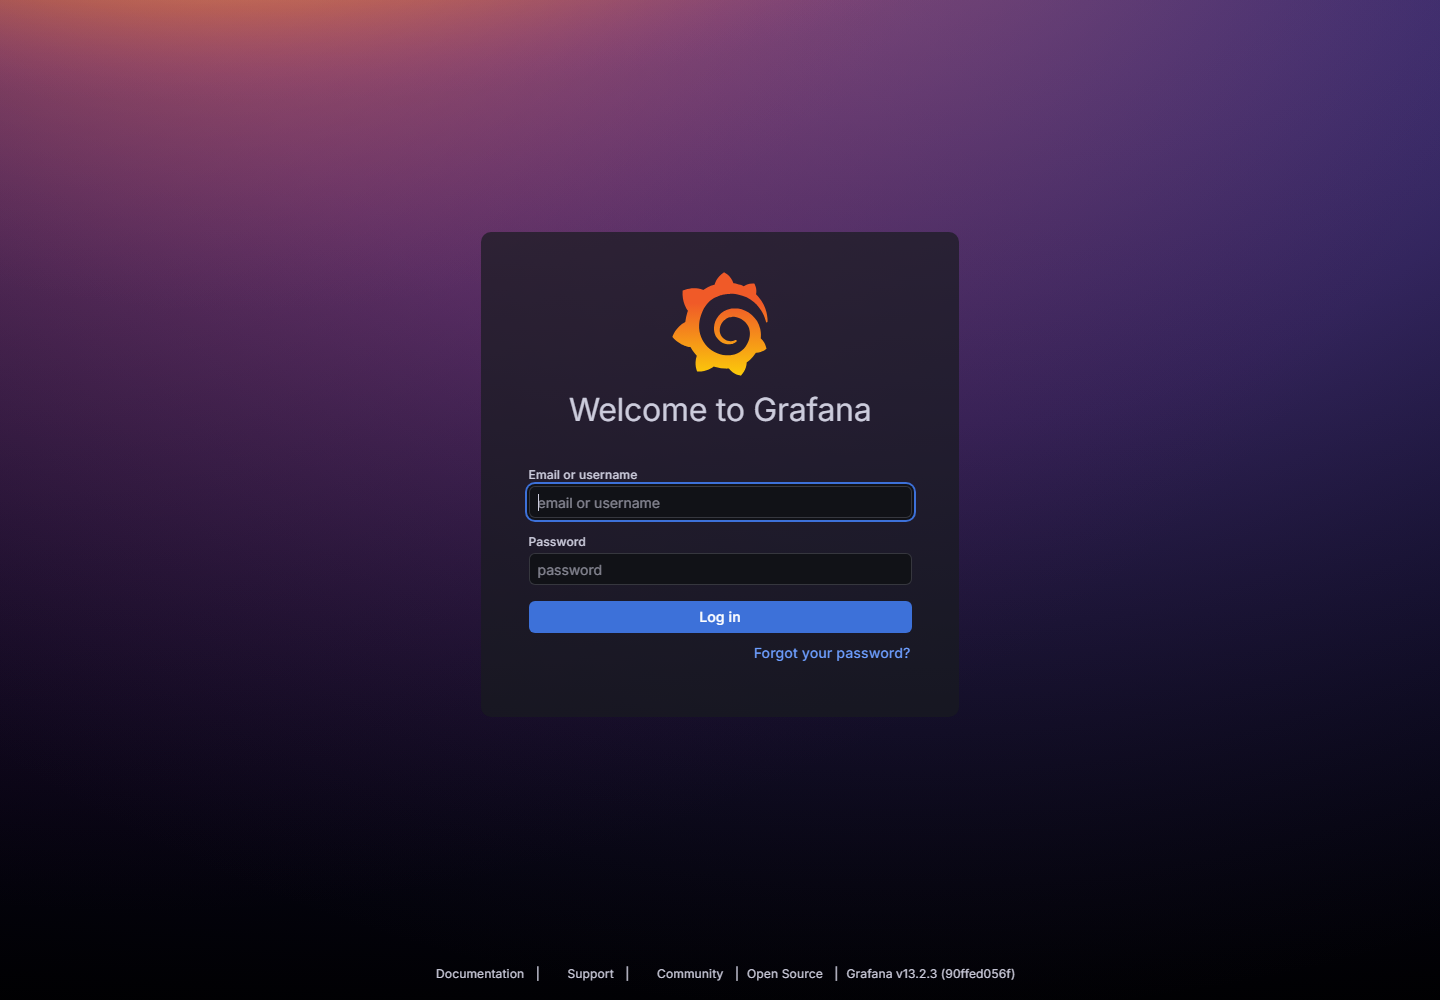
\includegraphics[width=0.9\linewidth]{evidence/03-grafana.png}
\caption{Instancia Grafana del stack de observabilidad desplegado en Kubernetes.}
\end{figure}

\section{Conclusiones}
La solución evidencia que los Pods son reemplazables, mientras el estado se conserva en
volúmenes persistentes. Services desacoplan clientes de direcciones efímeras; Deployments y
StatefulSets materializan el estado deseado; HPA adapta capacidad; y probes evitan enviar
tráfico a instancias no preparadas. Los experimentos convierten estas propiedades en
resultados visibles, medibles y repetibles.

\section{Trabajo futuro}
Como extensiones se propone incorporar Prometheus y Grafana para series temporales,
NetworkPolicy para segmentación explícita, External Secrets y CI/CD con publicación de
imágenes en un registro.

\end{document}
